\section{公式、图片、表格、伪代码与定理}
本节简单介绍如何本模版下插入公式、图片、表格与伪代码。
\subsection{公式}

公式可以分为行内公式与独立公式。行内公式是指公式与文字在同一行,独立公式是指公式与文字不在同一行。行内公式使用\$包围,独立公式使用\$\$或者$\backslash [ \backslash]$包围。比如下面的代码:

\begin{lstlisting}
设有对称矩阵的SVD分解为$\mathbf{X}=\mathbf{U}\mathbf{S}\mathbf{U}^{\mathrm{T}}$,那么
\[
    \mathbf{X}^{2} = \mathbf{U} \mathbf{S}^{2} \mathbf{U}^{\mathrm{T}}.
\]
\end{lstlisting}
对应的编译结果为:
\begin{shaded}
设有对称矩阵的SVD分解为$\mathbf{X}=\mathbf{U}\mathbf{S}\mathbf{U}^{\mathrm{T}}$,那么
\[
    \mathbf{X}^{2} = \mathbf{U} \mathbf{S}^{2} \mathbf{U}^{\mathrm{T}}
\]
\end{shaded}
如果需要对公式进行编号,可以使用$\backslash \text{begin\{equation\}} \dots \backslash \text{end\{equation\}}$包围公式,比如下面的代码:
\begin{lstlisting}
设有对称矩阵的SVD分解为$\mathbf{X}=\mathbf{U}\mathbf{S}\mathbf{U}^{\mathrm{T}}$,那么
\begin{equation}
    \mathbf{X}^{2} = \mathbf{U} \mathbf{S}^{2} \mathbf{U}^{\mathrm{T}}.
    \label{eq:1}
\end{equation}
\end{lstlisting}
其中$\backslash \text{label}$为公式的标签,在引用时会用到,具体的引用方法会在后面介绍。这段代码对应的编译结果为:
\begin{shaded}
设有对称矩阵的SVD分解为$\mathbf{X}=\mathbf{U}\mathbf{S}\mathbf{U}^{\mathrm{T}}$,那么
\begin{equation}
    \mathbf{X}^{2} = \mathbf{U} \mathbf{S}^{2} \mathbf{U}^{\mathrm{T}}.
    \label{eq:1}
\end{equation}
\end{shaded}


需要注意的是,一般矩阵需用大写字母,并且为加粗正体,即$\backslash \text{mathbf}$来修饰,例如$\mathbf{X},\mathbf{A}$。而向量使用小写字母,加粗斜体表示,在本模版中定义了$\backslash \text{bm}$指令来修饰向量,例如$\bm{x},\bm{a}$。

\subsection{图片}
图片的插入使用$\backslash \text{includegraphics}$指令,不过插入单张图片和多张图片的代码是不同的。插入单张图片的代码如下:
\begin{lstlisting}
\begin{figure}[htb!]
    \centering
    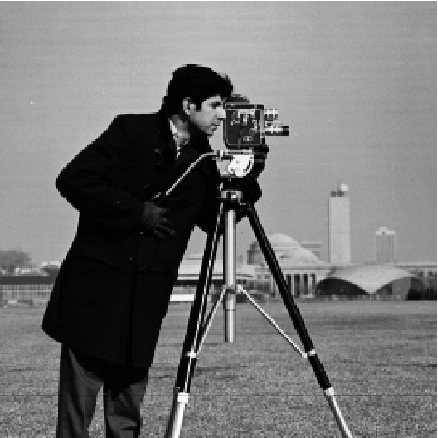
\includegraphics[width=.2\textwidth]{./img/im1.pdf}
    \caption{一幅图片}
    \label{fig:1}
\end{figure}
\end{lstlisting}

\begin{figure}[htb!]
    \centering
    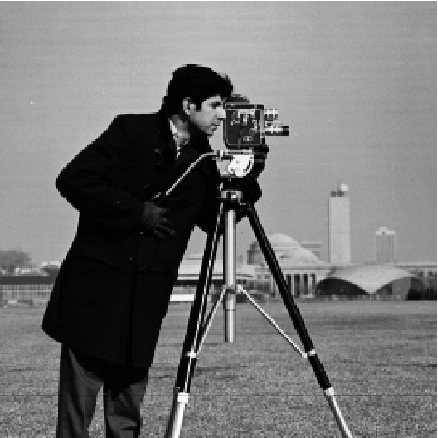
\includegraphics[width=.2\textwidth]{./img/im1.pdf}
    \caption{一幅图片}
    \label{fig:1}
\end{figure}

插入多张图片的代码如下:

\begin{lstlisting}
\begin{figure}[htb!]
    \centering
    \begin{subfigure}{.2\textwidth}
        \centering
        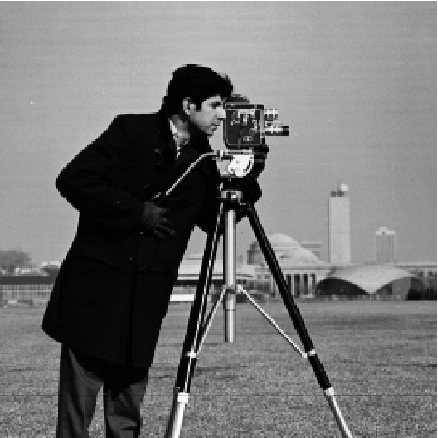
\includegraphics[width=\textwidth]{./img/im1.pdf}
        \caption{}
        \label{fig:cameraman2_1}
    \end{subfigure}
    \begin{subfigure}{.2\textwidth}
        \centering
        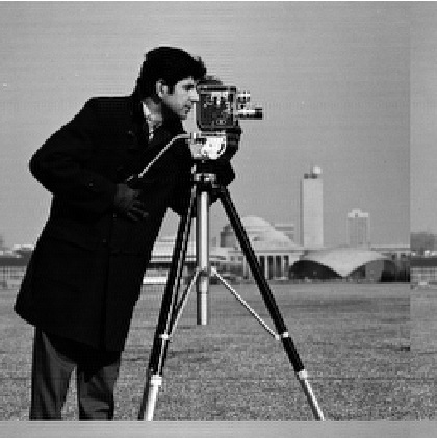
\includegraphics[width=\textwidth]{./img/im2.pdf}
        \caption{}
        \label{fig:cameraman2_2}
    \end{subfigure}
    
    \begin{subfigure}{.2\textwidth}
        \centering
        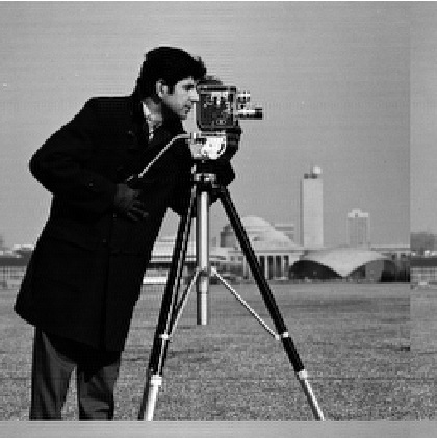
\includegraphics[width=\textwidth]{./img/im2.pdf}
        \caption{}
        \label{fig:cameraman2_3}
    \end{subfigure}
    \begin{subfigure}{.2\textwidth}
        \centering
        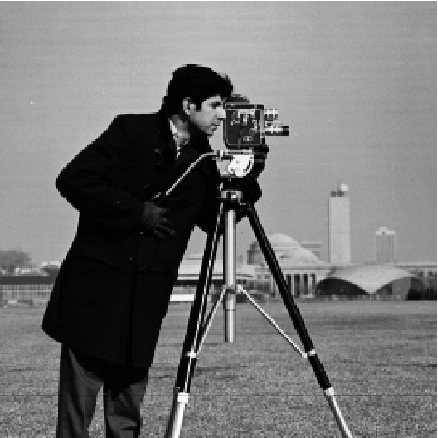
\includegraphics[width=\textwidth]{./img/im1.pdf}
        \caption{}
        \label{fig:cameraman2_4}
    \end{subfigure}
    \caption{两幅图片 (a) 原图像 (b) 平移后的图像 (c) 平移后的图像 (d) 原图像}
    \label{fig:cameraman2}
\end{figure}
\end{lstlisting}

\begin{figure}[htb!]
    \centering
    \begin{subfigure}{.2\textwidth}
        \centering
        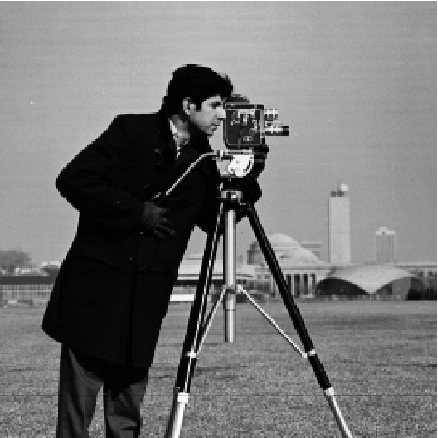
\includegraphics[width=\textwidth]{./img/im1.pdf}
        \caption{}
        \label{fig:cameraman2_1}
    \end{subfigure}
    \begin{subfigure}{.2\textwidth}
        \centering
        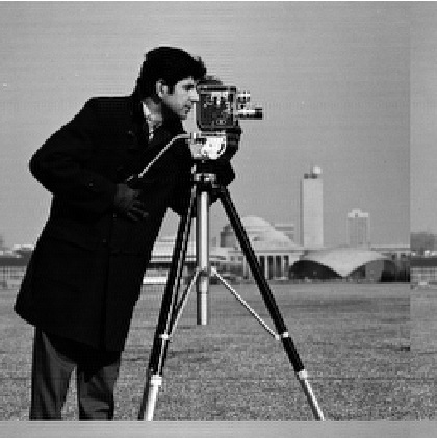
\includegraphics[width=\textwidth]{./img/im2.pdf}
        \caption{}
        \label{fig:cameraman2_2}
    \end{subfigure}

    \begin{subfigure}{.2\textwidth}
        \centering
        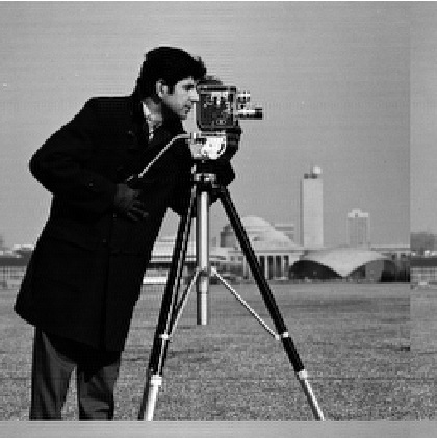
\includegraphics[width=\textwidth]{./img/im2.pdf}
        \caption{}
        \label{fig:cameraman2_3}
    \end{subfigure}
    \begin{subfigure}{.2\textwidth}
        \centering
        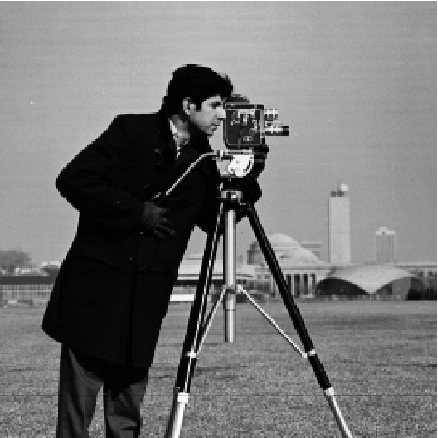
\includegraphics[width=\textwidth]{./img/im1.pdf}
        \caption{}
        \label{fig:cameraman2_4}
    \end{subfigure}
    \caption{两幅图片 (a) 原图像 (b) 平移后的图像 (c) 平移后的图像 (d) 原图像}
    \label{fig:cameraman2}
\end{figure}

\subsection{表格}

表格插入比较简单,具体的代码如下:
\begin{lstlisting}
\begin{table}[htbp!]
    \centering
    \caption{表格}
    \label{tab:1}
    \begin{tabular}{|c|c|c|}
        \hline
        \textbf{A} & \textbf{B} & \textbf{C} \\ \hline
        1 & 2 & 3 \\ \hline
        4 & 5 & 6 \\ \hline
        7 & 8 & 9 \\ \hline
    \end{tabular}
\end{table}
\end{lstlisting}
生成的表格如下:
\begin{table}[htb!]
    \centering
    \caption{表格}
    \label{tab:1}
    \begin{tabular}{|c|c|c|}
        \hline
        \textbf{A} & \textbf{B} & \textbf{C} \\ \hline
        1 & 2 & 3 \\ \hline
        4 & 5 & 6 \\ \hline
        7 & 8 & 9 \\ \hline
    \end{tabular}
\end{table}

推荐到在线表格生成网站\href{https://www.tablesgenerator.com/}{tablesgenerator}快速生成表格对应的LaTeX代码。

\subsection{伪代码}
伪代码部分使用了 algorithm 和 algorithmicx 宏包,对应的关键词需要全部大写,具体的代码如下:

\begin{lstlisting}
\begin{algorithm} 
    \caption{Calculate $y = |x|$} 
    \label{alg:1} 
    \begin{algorithmic}
        \REQUIRE $x$ 
        \ENSURE $y = |x|$ 
        \IF{$x \geq 0$} 
        \STATE $y = x$ 
        \ELSE 
        \STATE $y = -x$
        \ENDIF
    \end{algorithmic} 
\end{algorithm}
\end{lstlisting}
生成的伪代码见\cref{alg:1}。

\begin{algorithm} 
    \caption{Calculate $y = |x|$} 
    \label{alg:1} 
    \begin{algorithmic}
        \REQUIRE $x$ 
        \ENSURE $y = |x|$ 
        \IF{$x \geq 0$} 
        \STATE $y = x$ 
        \ELSE 
        \STATE $y = -x$
        \ENDIF
    \end{algorithmic} 
\end{algorithm}

\subsection{定理}
模版不仅仅支持定理,还支持引理、定义、证明等等,具体的代码如下:
\begin{lstlisting}
\begin{definition}
    这是一个定义。
    \label{def:1}
\end{definition}
\begin{lemma}
    这是一个引理。
    \label{lem:1}
\end{lemma}
\begin{theorem}
    这是一个定理。
    \label{thm:1}
\end{theorem}
\begin{proof}
    这是一个证明。
\end{proof}
\end{lstlisting}
编译结果如下:
\begin{shaded}
\begin{definition}
    这是一个定义。
    \label{def:1}
\end{definition}
\begin{lemma}
    这是一个引理。
    \label{lem:1}
\end{lemma}
\begin{theorem}
    这是一个定理。
    \label{thm:1}
\end{theorem}
\begin{proof}
    这是一个证明。
\end{proof}
\end{shaded}